\documentclass{report}
\usepackage[utf8]{inputenc}
\usepackage[francais]{babel}
\usepackage[T1]{fontenc}
\usepackage{lmodern}
\usepackage{ifpdf}
\usepackage{pdflscape} % ou lscape
\usepackage{graphicx}
\renewcommand{\familydefault}{\sfdefault}

\title{Guidage des étudiants par GPS sur le Campus Triolet, UM2 - Android}
\author{PAGÈS Julien \and SALEIL Baptiste \and BENGHABRIT Walid}
\date{\today}
\ifpdf
	\pdfinfo 
	{
		/Author (Pagès - Saleil - Benghabrit)
		/Title (Guidage des étudiants par GPS sur le Campus Triolet, UM2 - Android)
		/Subject (Guidage des étudiants par GPS sur le Campus Triolet)
		/Keywords ()
		/CreationDate (\today)
	}
\fi

\begin{document}
	% Page de titre
	\maketitle
	\thispagestyle{empty}
	
	\section*{Caractéristiques}
	\begin{itemize}
		\item Interface simple, rapide, intuitive \\
			Le but ici est de fournir la meilleure expérience possible a l'utilisateur. Tout doit être accessible rapidement car l'application doit etre utilisée souvent, mais rapidement.
		\item Barre d'outils permettant de rechercher \\
			Lorsque l'application est lancée, l'utiliateur doit pouvoir effectuer une recherche en un clic. L'idéal serait de proposer une autocomplétion sur les résultats connus. La bare d'outils doit également proposer les préférences essentielles comme recentrer la carte sur l'utilisateur, etc...
		\item Carte affichée au lancement avec focus sur l'UM2 \\
			La carte doit être affichée au lancement de l'application de manière à ce que l'utilisateur soit tout de suite informé de sa position au sein de l'université si disponible, ou centré sur l'université sinon.
	\end{itemize}

	\section*{Fonctionnalités}
	Ces fonctionnalités seront les premières implémentées car essentielles pour une telle application :
	\begin{itemize}
		\item Carte interactive
		\item Carte "annotée" avec les batiments, routes, etc...
		\item Liste brute des batiments ou l'utilisateur peut directement choisir son batiment.
		\item Guidage automatisé de l'utilisateur depuis sa position, vers la position souhaitée.
		\item Recherche textuelle / vocale permettant de rechercher un lieu le plus rapidement possible.
	\end{itemize}
	
	\section*{Fonctionnalités souhaitées}
	Ces fonctionnalités seront implémentées si le temps nous le permet :
	\begin{itemize}
		\item Points clés (Cafétéria, parkings, ...) répertoriés par l'application pour enrichir son contenu.
		\item Guidage vocal de l'utilisateur
		\item Synchronisation avec l'emploi du temps ADE, l'utilisateur sélectionne son cursus et son groupe, et n'a plus qu'à lancer l'application pour connaitre sa salle et diriger.
		\item Mode "plus court" / "plus accessible" notamment pour les personnes handicapées, qui ne peuvent pas forcément emprunter les chemins de terre pour se rendre à un batiment.
	\end{itemize}
	
	\section*{Vues}
	\begin{itemize}
	\item \textbf{Carte} : Affichage d'une carte en plein écran avec barre de menu pour préférences rapides. \\
	Voici une capture illustrant l'idée de notre application. Lorsque l'utilisateur lance l'application, la carte est l'élément affiché en premier. Une barre permet à l'utilisateur d'accéder aux fonctionnalités principales :  Recherche, Centrage,  etc... \\
		\begin{center}
			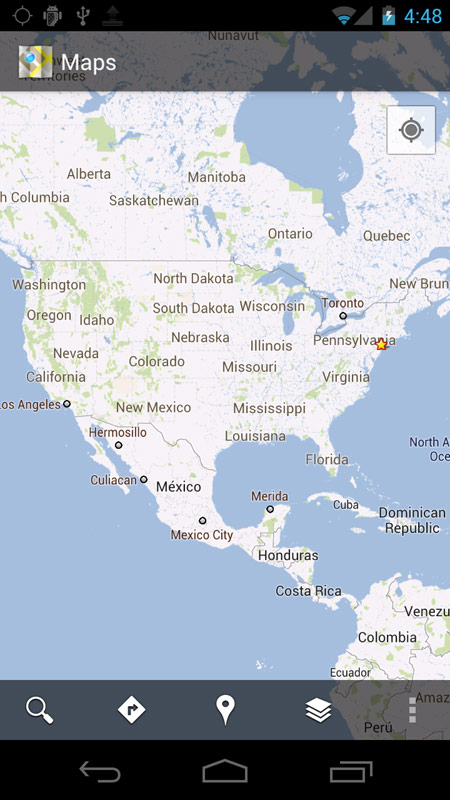
\includegraphics[scale=0.35]{map.jpg}
		\end{center}
	\item \textbf{Préférences} : Differents choix modifiant le comportement de l'application. \\
	La vue de présentation respectera le design et l'experience des menu classiques de préférences disponibles sur android avec cases à cocher ou autres widgets :
		\begin{center}
			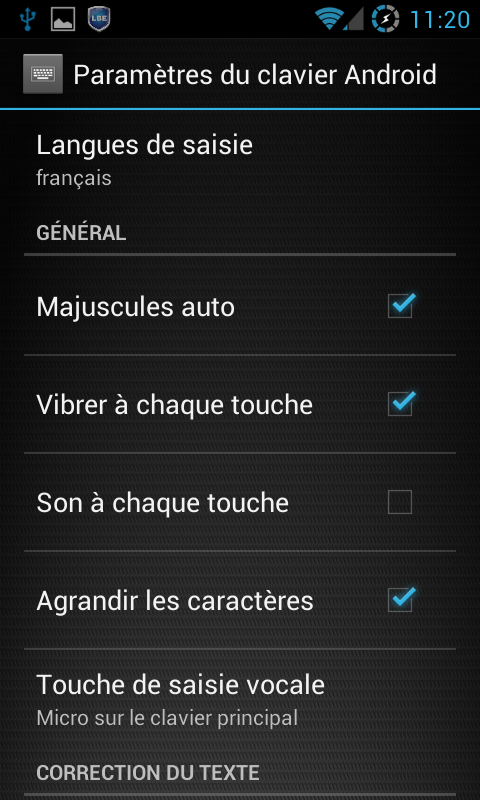
\includegraphics[scale=0.35]{preferences.png}
		\end{center}
	\item \textbf{Liste} : Choix lieu répertorié \\
	Cette vue permettra à l'utilisateur de parcourir l'ensemble des lieux répertoriés par l'application et éventuellement en choisir un.
	\end{itemize}
	
\end{document}
